\documentclass[11pt]{article}
\usepackage{../acl2016}

%\aclfinalcopy % Uncomment this line for the final submission
%\def\aclpaperid{***} %  Enter the acl Paper ID here
%\setlength\titlebox{5cm}
% You can expand the titlebox if you need extra space
% to show all the authors. Please do not make the titlebox
% smaller than 5cm (the original size); we will check this
% in the camera-ready version and ask you to change it back.

\usepackage[breaklinks, colorlinks, linkcolor=black, urlcolor=black, citecolor=black, draft]{hyperref}
\usepackage{natbib}
\usepackage{times}
\usepackage{latexsym}
% \setlength\titlebox{7.5cm}    % Expanding the titlebox

%%% Custom additions %%%
\usepackage{url}
\usepackage[leqno, fleqn]{amsmath}
\usepackage{amssymb}
\usepackage{qtree}
\usepackage{booktabs}
\usepackage{caption}
\usepackage{subcaption}
\usepackage{color}
\usepackage{tikz}
\usepackage{tikz-qtree}
\usepackage{pgfplots}
\usepackage{algorithm}
\usepackage[noend]{algpseudocode}
\usepackage{stmaryrd}
\usepackage{gb4e}

\newcommand\todo[1]{\textcolor{blue}{\textbf{TODO:} #1}}
\newcommand\result[1]{\textcolor{red}{\textbf{RESULT NEEDED:} #1}}
\newcommand\question[1]{\textcolor{orange}{\textbf{OPEN QUESTION:} #1}}

\newcount\colveccount
\newcommand*\colvec[1]{
        \global\colveccount#1
        \begin{bmatrix}
        \colvecnext
}
\def\colvecnext#1{
        #1
        \global\advance\colveccount-1
        \ifnum\colveccount>0
                \\
                \expandafter\colvecnext
        \else
                \end{bmatrix}
        \fi
}

\newcommand{\shift}{\textsc{shift}}
\newcommand{\reduce}{\textsc{reduce}}
 
\def\ii#1{\textit{#1}}
\newcommand{\word}[1]{\emph{#1}}
\newcommand{\fulllabel}[2]{\b{#1}\newline\textsc{#2}}

\newcommand{\snli}[3]{{\vspace{0.25em}
{\small \setlength{\parindent}{0.6em} \hangindent=1.2em  \textbf{Premise:} #1\par}\vspace{0.25em}
{\small \setlength{\parindent}{0.6em} \hangindent=1.2em   \textbf{Hypothesis:} #2\par}\vspace{0.25em}
{\small \setlength{\parindent}{0.6em}  \textbf{Label:} #3\par}
}}


\noautomath

\title{A Fast Unified Model for Parsing and Sentence Understanding} 

     \author{}
%    \author{
%    Samuel R.\ Bowman$^{1,2,5,}$\thanks{~\,The first two authors contributed equally.} \\
%    \texttt{\small sbowman@stanford.edu} \\
%    \And
%    Jon Gauthier$^{2,3,5,*}$ \\
%    \texttt{\small jgauthie@stanford.edu} \\
%    \And
%    Abhinav Rastogi$^{4,5}$ \\
%    \texttt{\small arastogi@stanford.edu} \\
%    \AND
%    Raghav Gupta$^{6}$ \\
%    \texttt{\small rgupta93@stanford.edu} \\
%    \And
%    Christopher D.\ Manning$^{1,2,5,6}$\\
%    \texttt{\small manning@stanford.edu}\\
%    \And
%    Christopher Potts$^{1}$\\
%    \texttt{\small cgpotts@stanford.edu}
%    \AND\\[-3ex]
%    {$^{1}$Stanford Linguistics\quad
%    $^{2}$Stanford NLP Group\quad
%    $^{3}$Stanford Symbolic Systems}\\
%    {$^{4}$Stanford Electrical Engineering\quad
%    $^{5}$Stanford AI Lab\quad
%    $^{6}$Stanford Computer Science}
%    }

\date{}


\begin{document}
\maketitle
\begin{abstract}

Tree-structured neural networks exploit valuable syntactic parse information as they interpret the meanings of sentences. However, they suffer from two key technical problems that make them slow and unwieldy for large-scale NLP tasks: they can only operate on parsed sentences and do not directly support batched computation. We address these issues by introducing the Stack-augmented Parser-Interpreter Neural Network (SPINN), which combines parsing and interpretation within a single tree-sequence hybrid model by integrating tree-structured sentence interpretation into the linear sequential structure of a shift-reduce parser. Our model supports batched computation for a speedup of up to 25x over other tree-structured models, and its integrated parser allows it to operate on unparsed data with nearly no loss of accuracy. We evaluate it on the Stanford NLI entailment task and show that it significantly outperforms other sentence encoding models.
\end{abstract}

\section{Introduction}

%!TEX root = paper.tex

\begin{figure}[t]

\begin{subfigure}[t]{\columnwidth}
 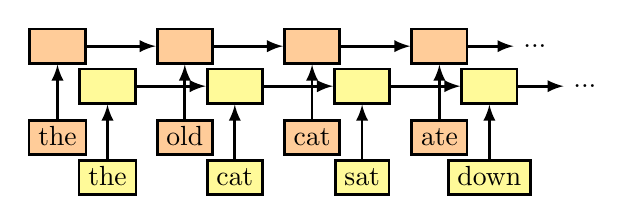
\begin{tikzpicture}
    \tikzstyle{word}=[fill=yellow!40,text height=2mm,line width=1pt,draw=black]    
    \tikzstyle{nonleaf}=[fill=yellow!40,text height=2mm,line width=1pt,draw=black] 
    \tikzstyle{alt}=[fill=orange!40]
    \pgfsetarrowsend{latex}
    \tikzstyle{fwd} = [draw=black, line width=1pt]
   
    \def\dx{23pt}
    \def\dy{11pt}
    \def\sy{7*\dy}
    \def\oxb{5.5*\dx}
    \def\by{1*\dy}
    \def\ox{0*\oxb}


    \begin{scope}[shift={(0in,0in)}, frontier/.style={distance from root=60pt}]
    
    \node[word,alt]  (w1) at (\ox+-3*\dx,\by+0*\dy) {the};
    \node[word,alt]  (w2) at (\ox+-1*\dx,\by+0*\dy) {old};
    \node[word,alt]  (w3) at (\ox+1*\dx,\by+0*\dy) {cat};
    \node[word,alt]  (w4) at (\ox+3*\dx,\by+0*\dy) {ate};

    \node[word,alt]  (n1) at (\ox+-3*\dx,\by+3*\dy) {~~~~~};
    \node[word,alt]  (n2) at (\ox+-1*\dx,\by+3*\dy) {~~~~~};
    \node[word,alt]  (n3) at (\ox+1*\dx,\by+3*\dy) {~~~~~};
    \node[word,alt]  (n4) at (\ox+3*\dx,\by+3*\dy) {~~~~~};
    \node[]  (n5) at (\ox+4.5*\dx,\by+3*\dy) {...};

   \draw [fwd] (w1) -- (n1);
   \draw [fwd] (w2) -- (n2);
   \draw [fwd] (w3) -- (n3);
   \draw [fwd] (w4) -- (n4);

   \draw [fwd] (n1) -- (n2);
   \draw [fwd] (n2) -- (n3);
   \draw [fwd] (n3) -- (n4);
   \draw [fwd] (n4) -- (n5);


    \end{scope}

    \begin{scope}[shift={(0.25in,-0.2in)}, frontier/.style={distance from root=60pt}]
    
    \node[word]  (w1) at (\ox+-3*\dx,\by+0*\dy) {the};
    \node[word]  (w2) at (\ox+-1*\dx,\by+0*\dy) {cat};
    \node[word]  (w3) at (\ox+1*\dx,\by+0*\dy) {sat};
    \node[word]  (w4) at (\ox+3*\dx,\by+0*\dy) {down};

    \node[word]  (n1) at (\ox+-3*\dx,\by+3*\dy) {~~~~~};
    \node[word]  (n2) at (\ox+-1*\dx,\by+3*\dy) {~~~~~};
    \node[word]  (n3) at (\ox+1*\dx,\by+3*\dy) {~~~~~};
    \node[word]  (n4) at (\ox+3*\dx,\by+3*\dy) {~~~~~};
    \node[]  (n5) at (\ox+4.5*\dx,\by+3*\dy) {...};


   \draw [fwd] (w1) -- (n1);
   \draw [fwd] (w2) -- (n2);
   \draw [fwd] (w3) -- (n3);
   \draw [fwd] (w4) -- (n4);

   \draw [fwd] (n1) -- (n2);
   \draw [fwd] (n2) -- (n3);
   \draw [fwd] (n3) -- (n4);
   \draw [fwd] (n4) -- (n5);

    \end{scope}

\end{tikzpicture}


\caption{\label{fig:batching:good}A conventional sequence-based RNN, instantiated for two sentences.}
\end{subfigure}

\vspace{2em}

\begin{subfigure}[t]{\columnwidth}
\begin{center}
 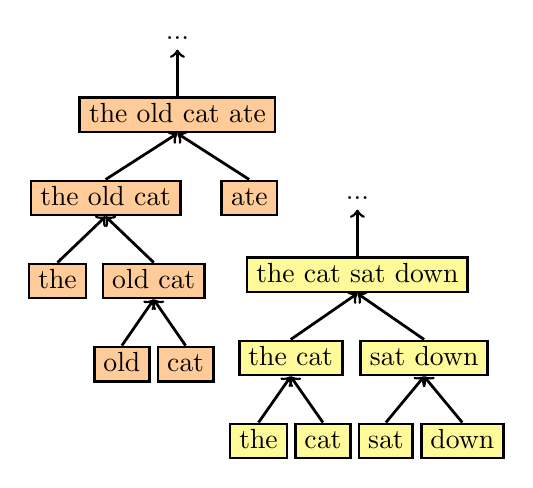
\begin{tikzpicture}
    \tikzstyle{word}=[fill=yellow!40,text height=2mm,line width=1pt,draw=black]    
    \tikzstyle{nonleaf}=[fill=yellow!40,text height=2mm,line width=1pt,draw=black]
    \tikzstyle{alt}=[fill=orange!40]    
    \pgfsetarrowsend{latex}
    \tikzset{edge from parent/.append style={<-, line width=1pt}}   

    \begin{scope}[shift={(0in,0in)}]

    \Tree [.\node[](root){...}; [.\node[nonleaf,alt](2thekittenate){the old cat ate}; [.\node[nonleaf,alt](2thekitten){the old cat}; \node[word,alt](2the){the}; [.\node[nonleaf,alt](2bigkitten){old cat}; \node[word,alt](2kitten){old}; \node[word,alt](2kitten){cat}; ] ] \node[word,alt](2ate){ate}; ] ]

    \end{scope}


    \begin{scope}[shift={(0.9in,-0.8in)}]

    \Tree [.\node[](root){...}; [.\node[nonleaf](1thecatsatdown){the cat sat down}; [.\node[nonleaf](1thecat){the cat}; \node[word](1the){the}; \node[word](1cat){cat}; ] [.\node[nonleaf](1satdown){sat down}; \node[word](1sat){sat}; \node[word](1down){down}; ] ] ]

    \end{scope}

\end{tikzpicture}
\end{center}

\caption{\label{fig:batching:bad}A conventional TreeRNN, instantiated for two sentences.}
\end{subfigure}

\caption{An illustration of two standard designs for sentence encoders. Note that the TreeRNN, unlike the sequence-based RNN, requires a substantially different connection structure for each sentence.}
\end{figure}


\begin{figure*}[t]
\begin{subfigure}[t]{\textwidth}
\centering
\scalebox{0.6}{
 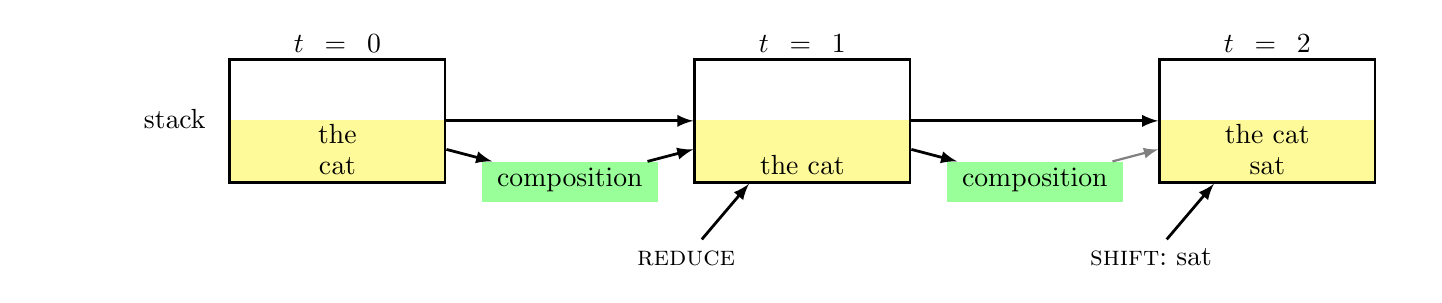
\begin{tikzpicture}
    \def\dx{21pt}
    \def\dy{11pt}
    \def\sy{13*\dy}
    \def\oxb{8*\dx}
    \def\by{1*\dy}
    \def\ox{0*\oxb}

    \tikzstyle{label}=[text width=35mm,align=center,text height=2mm]    
    \tikzstyle{word}=[text width=35mm,align=center,text height=2mm]    
    \tikzstyle{comp}=[fill=green!40,text width=20mm,align=center,text height=2mm]
    \tikzstyle{input}=[line width=1pt,text width=20mm,align=center,text height=2mm]    
    \tikzstyle{sbox}=[line width=1pt,draw=black,text width=25mm,align=center,text height=13.3mm]
    \tikzstyle{bbox}=[line width=1pt,draw=black,text width=25mm,align=center,text height=6.5mm]
    \tikzstyle{focus1}=[fill=yellow!80,opacity=0.5,text width=25mm,align=center,text height=2mm]
    \tikzstyle{focus2}=[fill=yellow!80,opacity=0.5,text width=25mm,align=center,text height=5.5mm]
    
    \node[label]  (sl) at (\ox-0.35*\oxb+0*\dx,\sy+0.5*\dy) {stack};
    
    \node[label]  (1l) at (\ox+0*\dx,\sy+3*\dy) {$t=0$};
    
    \node[focus2] (0sb) at  (\ox+0*\dx,\sy-0.5*\dy) {};
    \node[word]  (0s1) at (\ox+0*\dx,\sy-1*\dy) {cat};
    \node[word]  (0s2) at (\ox+0*\dx,\sy+0*\dy) {the};
    \node[word]  (0s3) at (\ox+0*\dx,\sy+1*\dy) {};
    \node[sbox] (0sb) at  (\ox+0*\dx,\sy+0.5*\dy) {};
    
    \node[comp] (0c) at  (\ox+0.5*\oxb,\sy-1.5*\dy) {composition};
    
    \node[input] (0so) at  (\ox+0.75*\oxb,9*\dy) {\reduce};
    
    \def\ox{1*\oxb}
    
    \node[label]  (1l) at (\ox+0*\dx,\sy+3*\dy) {$t=1$};
    
    \node[focus2] (1sb) at  (\ox+0*\dx,\sy-0.5*\dy) {};
    \node[word]  (1s1) at (\ox+0*\dx,\sy-1*\dy) {the cat};
    \node[word]  (1s2) at (\ox+0*\dx,\sy+0*\dy) {};
    \node[word]  (1s3) at (\ox+0*\dx,\sy+1*\dy) {};
    \node[sbox] (1sb) at  (\ox+0*\dx,\sy+0.5*\dy) {};
    
    \node[comp] (1c) at  (\ox+0.5*\oxb,\sy-1.5*\dy) {composition};
    
    \node[input] (1so) at  (\ox+0.75*\oxb,9*\dy) {\shift:~sat};
     
    \def\ox{2*\oxb}

    \node[label]  (1l) at (\ox+0*\dx,\sy+3*\dy) {$t=2$};

    \node[focus2] (2sb) at  (\ox+0*\dx,\sy-0.5*\dy) {};
    \node[word]  (2s1) at (\ox+0*\dx,\sy-1*\dy) {sat};
    \node[word]  (2s2) at (\ox+0*\dx,\sy+0*\dy) {the cat};
    \node[word]  (2s3) at (\ox+0*\dx,\sy+1*\dy) {};
    \node[sbox] (2sb) at  (\ox+0*\dx,\sy+0.5*\dy) {};
  
   
    \pgfsetarrowsend{latex}
    \tikzstyle{fwd} = [draw=black, line width=1pt]
    \tikzstyle{gated} = [draw=black!50, line width=0.8pt]

    \draw [fwd] (0sb) -- (0c);
    
    \draw [fwd] (0sb) -- (1sb);
    \draw [fwd] (0so) -- (1sb);
    \draw [fwd] (0c) -- (1sb);

    \draw [fwd] (1sb) -- (1c);
    
    \draw [fwd] (1sb) -- (2sb);
    \draw [fwd] (1so) -- (2sb);
    \draw [gated] (1c) -- (2sb);




  \end{tikzpicture}}
  
 \caption{\label{fig:model:0}The Model 0 network unrolled for two transitions on the input \word{the cat sat down}. The operations at the bottom of the figure are given as inputs to the models, as is the start state of the stack at $t=0$.}
  
\end{subfigure}\\\\\\
\begin{subfigure}[t]{\textwidth}
\centering
\scalebox{0.6}{
 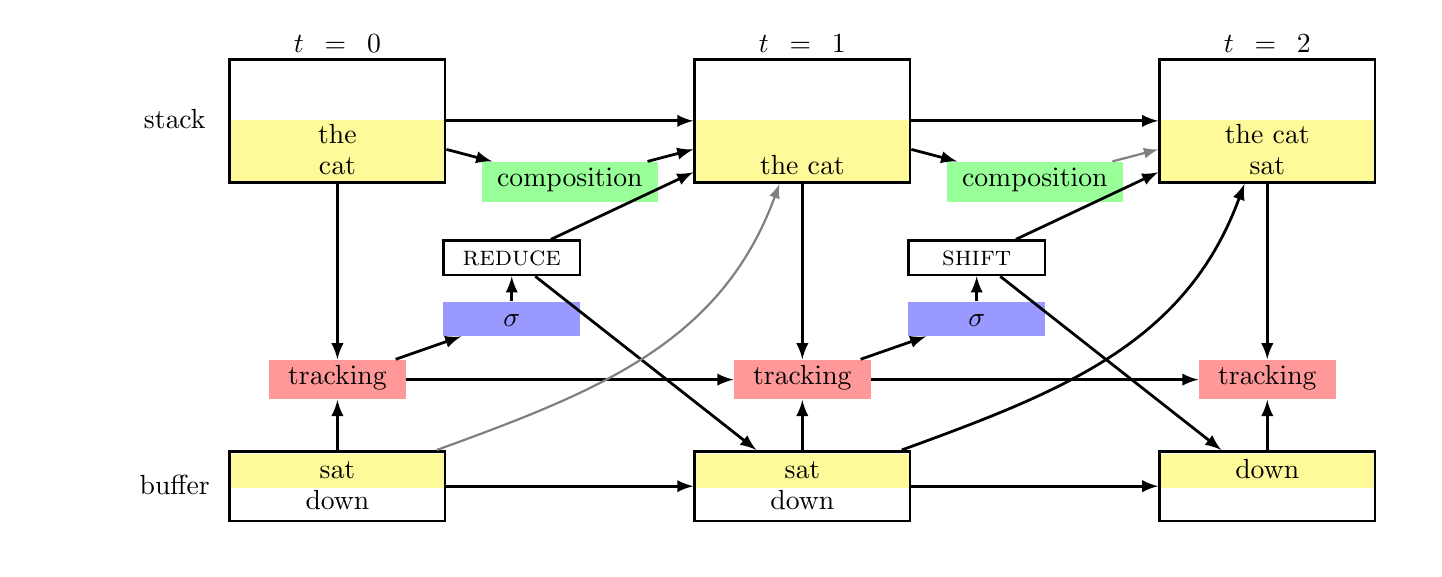
\begin{tikzpicture}
    \def\dx{21pt}
    \def\dy{11pt}
    \def\sy{13*\dy}
    \def\oxb{8*\dx}
    \def\by{1*\dy}
    \def\ox{0*\oxb}

    \tikzstyle{label}=[text width=35mm,align=center,text height=2mm]    
    \tikzstyle{word}=[text width=35mm,align=center,text height=2mm]    
    \tikzstyle{tracker}=[fill=red!40,text width=15mm,align=center,text height=2mm]
    \tikzstyle{softmax}=[fill=blue!40,text width=15mm,align=center,text height=2mm]
    \tikzstyle{comp}=[fill=green!40,text width=20mm,align=center,text height=2mm]
    \tikzstyle{result}=[line width=1pt,draw=black,text width=15mm,align=center,text height=2mm]    
    \tikzstyle{sbox}=[line width=1pt,draw=black,text width=25mm,align=center,text height=13.3mm]
    \tikzstyle{bbox}=[line width=1pt,draw=black,text width=25mm,align=center,text height=6.5mm]
    \tikzstyle{focus1}=[fill=yellow!80,opacity=0.5,text width=25mm,align=center,text height=2mm]
    \tikzstyle{focus2}=[fill=yellow!80,opacity=0.5,text width=25mm,align=center,text height=5.5mm]

    \node[label]  (sl) at (\ox-0.35*\oxb+0*\dx,\by+0.5*\dy) {buffer};

    \node[label]  (1l) at (\ox+0*\dx,\sy+3*\dy) {$t=0$};

    \node[focus1] (0bb) at  (\ox+0*\dx,2*\dy) {};
    \node[word]  (0b3) at (\ox+0*\dx,\by-1*\dy) {};
    \node[word]  (0b2) at (\ox+0*\dx,\by+0*\dy) {down};
    \node[word]  (0b1) at (\ox+0*\dx,\by+1*\dy) {sat};
    \node[bbox] (0bb) at  (\ox+0*\dx,\by+0.5*\dy) {};
    
    \node[label]  (sl) at (\ox-0.35*\oxb+0*\dx,\sy+0.5*\dy) {stack};
    
    \node[focus2] (0sb) at  (\ox+0*\dx,\sy-0.5*\dy) {};
    \node[word]  (0s1) at (\ox+0*\dx,\sy-1*\dy) {cat};
    \node[word]  (0s2) at (\ox+0*\dx,\sy+0*\dy) {the};
    \node[word]  (0s3) at (\ox+0*\dx,\sy+1*\dy) {};
    \node[sbox] (0sb) at  (\ox+0*\dx,\sy+0.5*\dy) {};
    
    \node[comp] (0c) at  (\ox+0.5*\oxb,\sy-1.5*\dy) {composition};
    
    \node[tracker] (0t) at  (\ox+0*\dx,5*\dy) {tracking};
    \node[softmax] (0sm) at  (\ox+3*\dx,7*\dy) {$\sigma$};
    \node[result] (0so) at  (\ox+3*\dx,9*\dy) {\reduce};
    
    \def\ox{1*\oxb}

    \node[label]  (1l) at (\ox+0*\dx,\sy+3*\dy) {$t=1$};

    \node[focus1] (1bb) at  (\ox+0*\dx,2*\dy) {};
    \node[word]  (1b3) at (\ox+0*\dx,\by-1*\dy) {};
    \node[word]  (1b2) at (\ox+0*\dx,\by+0*\dy) {down};
    \node[word]  (1b1) at (\ox+0*\dx,\by+1*\dy) {sat};
    \node[bbox] (1bb) at  (\ox+0*\dx,\by+0.5*\dy) {};
    
    \node[focus2] (1sb) at  (\ox+0*\dx,\sy-0.5*\dy) {};
    \node[word]  (1s1) at (\ox+0*\dx,\sy-1*\dy) {the cat};
    \node[word]  (1s2) at (\ox+0*\dx,\sy+0*\dy) {};
    \node[word]  (1s3) at (\ox+0*\dx,\sy+1*\dy) {};
    \node[sbox] (1sb) at  (\ox+0*\dx,\sy+0.5*\dy) {};
    
    \node[comp] (1c) at  (\ox+0.5*\oxb,\sy-1.5*\dy) {composition};
    
    \node[tracker] (1t) at  (\ox+0*\dx,5*\dy) {tracking};
    \node[softmax] (1sm) at  (\ox+3*\dx,7*\dy) {$\sigma$};
    \node[result] (1so) at  (\ox+3*\dx,9*\dy) {\shift};
     
    \def\ox{2*\oxb}

    \node[label]  (1l) at (\ox+0*\dx,\sy+3*\dy) {$t=2$};

    \node[focus1] (2bb) at  (\ox+0*\dx,2*\dy) {};
    \node[word]  (2b3) at (\ox+0*\dx,\by-1*\dy) {};
    \node[word]  (2b2) at (\ox+0*\dx,\by+0*\dy) {};
    \node[word]  (2b1) at (\ox+0*\dx,\by+1*\dy) {down};
    \node[bbox] (2bb) at  (\ox+0*\dx,\by+0.5*\dy) {};
    
    \node[focus2] (2sb) at  (\ox+0*\dx,\sy-0.5*\dy) {};
    \node[word]  (2s1) at (\ox+0*\dx,\sy-1*\dy) {sat};
    \node[word]  (2s2) at (\ox+0*\dx,\sy+0*\dy) {the cat};
    \node[word]  (2s3) at (\ox+0*\dx,\sy+1*\dy) {};
    \node[sbox] (2sb) at  (\ox+0*\dx,\sy+0.5*\dy) {};
   
    \node[tracker] (2t) at  (\ox+0*\dx,5*\dy) {tracking};

    
    \pgfsetarrowsend{latex}
    \tikzstyle{fwd} = [draw=black, line width=1pt]
    \tikzstyle{gated} = [draw=black!50, line width=0.8pt]

    \draw [fwd] (0sb) -- (0t);
    \draw [fwd] (0bb) -- (0t);
    \draw [fwd] (0t) -- (0sm);
    \draw [fwd] (0sm) -- (0so);
    \draw [fwd] (0sb) -- (0c);
    
    \draw [fwd] (0t) -- (1t);
    \draw [fwd] (0sb) -- (1sb);
    \draw [fwd] (0bb) -- (1bb);
    \draw [fwd] (0so) -- (1sb);
    \draw [fwd] (0so) -- (1bb);
    \draw [gated] (0bb) to[out=20,in=-110] (1sb);
    \draw [fwd] (0c) -- (1sb);

    \draw [fwd] (1sb) -- (1t);
    \draw [fwd] (1bb) -- (1t);
    \draw [fwd] (1t) -- (1sm);
    \draw [fwd] (1sm) -- (1so);
    \draw [fwd] (1sb) -- (1c);
    
    \draw [fwd] (1t) -- (2t);
    \draw [fwd] (1sb) -- (2sb);
    \draw [fwd] (1bb) -- (2bb);
    \draw [fwd] (1so) -- (2sb);
    \draw [fwd] (1so) -- (2bb);
    \draw [fwd] (1bb) to[out=20,in=-110] (2sb);
    \draw [gated] (1c) -- (2sb);

    \draw [fwd] (2sb) -- (2t);
    \draw [fwd] (2bb) -- (2t);


  \end{tikzpicture}}
  
 \caption{The Model 1/2 network unrolled for two transitions on the input \word{the cat sat down}. The start state of the stack and buffer at the initial step $t=0$ are the sole inputs to the model.}\label{fig:model:1d}
  
\end{subfigure}\\\\\\
\begin{subfigure}[t]{\textwidth}
\centering
\scalebox{0.6}{
 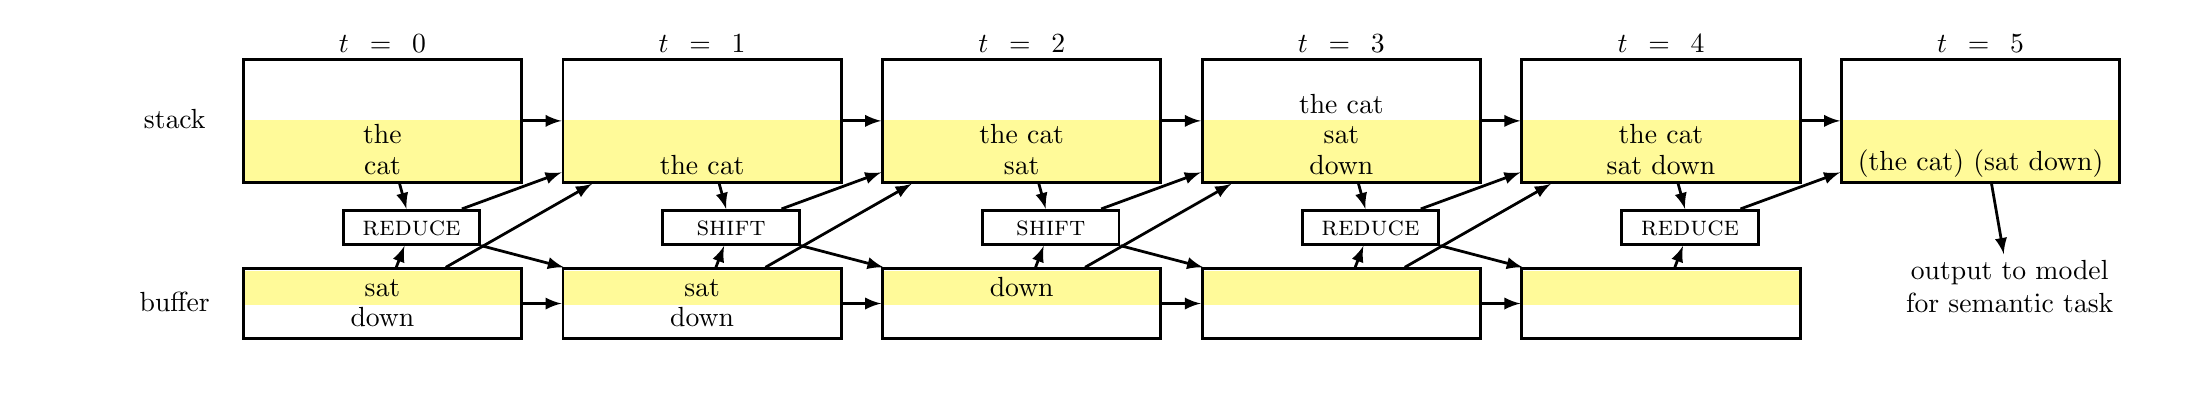
\begin{tikzpicture}
    \def\dx{21pt}
    \def\dy{11pt}
    \def\sy{7*\dy}
    \def\oxb{5.5*\dx}
    \def\by{1*\dy}
    \def\ox{0*\oxb}

    \tikzstyle{label}=[text width=35mm,align=center,text height=2mm]    
    \tikzstyle{word}=[text width=35mm,align=center,text height=2mm]    
    \tikzstyle{tracker}=[fill=red!40,text width=15mm,align=center,text height=2mm]
    \tikzstyle{softmax}=[text width=40mm,align=center,text height=2mm]
    \tikzstyle{comp}=[fill=green!40,text width=20mm,align=center,text height=2mm]
    \tikzstyle{result}=[line width=1pt,draw=black,text width=15mm,align=center,text height=2mm]    
    \tikzstyle{sbox}=[line width=1pt,draw=black,text width=33mm,align=center,text height=13.3mm]
    \tikzstyle{bbox}=[line width=1pt,draw=black,text width=33mm,align=center,text height=6.5mm]
    \tikzstyle{focus1}=[fill=yellow!80,opacity=0.5,text width=33mm,align=center,text height=2mm]
    \tikzstyle{focus2}=[fill=yellow!80,opacity=0.5,text width=33mm,align=center,text height=5.5mm]

    \def\ox{0*\oxb}
    
    \node[label]  (1l) at (\ox+0*\dx,\sy+3*\dy) {$t=0$};
    
    \node[label]  (sl) at (\ox-0.65*\oxb+0*\dx,\by+0.5*\dy) {buffer};
    
    \node[focus1] (1bb) at  (\ox+0*\dx,2*\dy) {};
    \node[word]  (1b3) at (\ox+0*\dx,\by-1*\dy) {};
    \node[word]  (1b2) at (\ox+0*\dx,\by+0*\dy) {down};
    \node[word]  (1b1) at (\ox+0*\dx,\by+1*\dy) {sat};
    \node[bbox] (1bb) at  (\ox+0*\dx,\by+0.5*\dy) {};
    
    \node[label]  (sl) at (\ox-0.65*\oxb+0*\dx,\sy+0.5*\dy) {stack};
    
    \node[focus2] (1sb) at  (\ox+0*\dx,\sy-0.5*\dy) {};
    \node[word]  (1s1) at (\ox+0*\dx,\sy-1*\dy) {cat};
    \node[word]  (1s2) at (\ox+0*\dx,\sy+0*\dy) {the};
    \node[word]  (1s3) at (\ox+0*\dx,\sy+1*\dy) {};
    \node[sbox] (1sb) at  (\ox+0*\dx,\sy+0.5*\dy) {};
    
    \node[result] (1so) at  (\ox+0.5*\dx,4*\dy) {\reduce};
              
    \def\ox{1*\oxb}
   
    \node[label]  (1l) at (\ox+0*\dx,\sy+3*\dy) {$t=1$};
    
    \node[focus1] (2bb) at  (\ox+0*\dx,2*\dy) {};
    \node[word]  (2b3) at (\ox+0*\dx,\by-1*\dy) {};
    \node[word]  (2b2) at (\ox+0*\dx,\by+0*\dy) {down};
    \node[word]  (2b1) at (\ox+0*\dx,\by+1*\dy) {sat};
    \node[bbox] (2bb) at  (\ox+0*\dx,\by+0.5*\dy) {};
    
    \node[focus2] (2sb) at  (\ox+0*\dx,\sy-0.5*\dy) {};
    \node[word]  (2s1) at (\ox+0*\dx,\sy-1*\dy) {the cat};
    \node[word]  (2s2) at (\ox+0*\dx,\sy+0*\dy) {};
    \node[word]  (2s3) at (\ox+0*\dx,\sy+1*\dy) {};
    \node[sbox] (2sb) at  (\ox+0*\dx,\sy+0.5*\dy) {};
    
    \node[result] (2so) at  (\ox+0.5*\dx,4*\dy) {\shift};
             
    \def\ox{2*\oxb}
    
    \node[label]  (1l) at (\ox+0*\dx,\sy+3*\dy) {$t=2$};
    
    \node[focus1] (3bb) at  (\ox+0*\dx,2*\dy) {};
    \node[word]  (3b3) at (\ox+0*\dx,\by-1*\dy) {};
    \node[word]  (3b2) at (\ox+0*\dx,\by+0*\dy) {};
    \node[word]  (3b1) at (\ox+0*\dx,\by+1*\dy) {down};
    \node[bbox] (3bb) at  (\ox+0*\dx,\by+0.5*\dy) {};
    
    \node[focus2] (3sb) at  (\ox+0*\dx,\sy-0.5*\dy) {};
    \node[word]  (3s1) at (\ox+0*\dx,\sy-1*\dy) {sat};
    \node[word]  (3s2) at (\ox+0*\dx,\sy+0*\dy) {the cat};
    \node[word]  (3s3) at (\ox+0*\dx,\sy+1*\dy) {};
    \node[sbox] (3sb) at  (\ox+0*\dx,\sy+0.5*\dy) {};
    
    \node[result] (3so) at  (\ox+0.5*\dx,4*\dy) {\shift};

    \def\ox{3*\oxb}
    
    \node[label]  (1l) at (\ox+0*\dx,\sy+3*\dy) {$t=3$};
        
    \node[focus1] (4bb) at  (\ox+0*\dx,2*\dy) {};
    \node[word]  (4b3) at (\ox+0*\dx,\by-1*\dy) {};
    \node[word]  (4b2) at (\ox+0*\dx,\by+0*\dy) {};
    \node[word]  (4b1) at (\ox+0*\dx,\by+1*\dy) {};
    \node[bbox] (4bb) at  (\ox+0*\dx,\by+0.5*\dy) {};
    
    \node[focus2] (4sb) at  (\ox+0*\dx,\sy-0.5*\dy) {};
    \node[word]  (4s1) at (\ox+0*\dx,\sy-1*\dy) {down};
    \node[word]  (4s2) at (\ox+0*\dx,\sy+0*\dy) {sat};
    \node[word]  (4s3) at (\ox+0*\dx,\sy+1*\dy) {the cat};
    \node[sbox] (4sb) at  (\ox+0*\dx,\sy+0.5*\dy) {};
    
    \node[result] (4so) at  (\ox+0.5*\dx,4*\dy) {\reduce};
                  
    \def\ox{4*\oxb}
    
    \node[label]  (1l) at (\ox+0*\dx,\sy+3*\dy) {$t=4$};
    
    \node[focus1] (5bb) at  (\ox+0*\dx,2*\dy) {};
    \node[word]  (5b3) at (\ox+0*\dx,\by-1*\dy) {};
    \node[word]  (5b2) at (\ox+0*\dx,\by+0*\dy) {};
    \node[word]  (5b1) at (\ox+0*\dx,\by+1*\dy) {};
    \node[bbox] (5bb) at  (\ox+0*\dx,\by+0.5*\dy) {};
    
    \node[focus2] (5sb) at  (\ox+0*\dx,\sy-0.5*\dy) {};
    \node[word]  (5s1) at (\ox+0*\dx,\sy-1*\dy) {sat down};
    \node[word]  (5s2) at (\ox+0*\dx,\sy+0*\dy) {the cat};
    \node[word]  (5s3) at (\ox+0*\dx,\sy+1*\dy) {};
    \node[sbox] (5sb) at  (\ox+0*\dx,\sy+0.5*\dy) {};
    
    \node[result] (5so) at  (\ox+0.5*\dx,4*\dy) {\reduce};
    
    \def\ox{5*\oxb}

    \node[label]  (1l) at (\ox+0*\dx,\sy+3*\dy) {$t=5$};

    \node[focus2] (6sb) at  (\ox+0*\dx,\sy-0.5*\dy) {};
    \node[word]  (6s1) at (\ox+0*\dx,\sy-1*\dy) {(the cat) (sat down)};
    \node[word]  (6s2) at (\ox+0*\dx,\sy+0*\dy) {};
    \node[word]  (6s3) at (\ox+0*\dx,\sy+1*\dy) {};
    \node[sbox] (6sb) at  (\ox+0*\dx,\sy+0.5*\dy) {};

    \node[softmax] (6sm) at  (\ox+0.5*\dx,2*\dy) {output to model for semantic task};
                   
    \pgfsetarrowsend{latex}
    \tikzstyle{fwd} = [draw=black, line width=1pt]

   \draw [fwd] (1sb) -- (1so);
   \draw [fwd] (1bb) -- (1so);

    \draw [fwd] (1sb) -- (2sb);
    \draw [fwd] (1bb) -- (2bb);
    \draw [fwd] (1so) -- (2sb);
    \draw [fwd] (1so) -- (2bb);
    \draw [fwd] (1bb) -- (2sb);

   \draw [fwd] (2sb) -- (2so);
   \draw [fwd] (2bb) -- (2so);

    \draw [fwd] (2sb) -- (3sb);
    \draw [fwd] (2bb) -- (3bb);
    \draw [fwd] (2so) -- (3sb);
    \draw [fwd] (2so) -- (3bb);
    \draw [fwd] (2bb) -- (3sb);

   \draw [fwd] (3sb) -- (3so);
   \draw [fwd] (3bb) -- (3so);

    \draw [fwd] (3sb) -- (4sb);
    \draw [fwd] (3bb) -- (4bb);
    \draw [fwd] (3so) -- (4sb);
    \draw [fwd] (3so) -- (4bb);
    \draw [fwd] (3bb) -- (4sb);

   \draw [fwd] (4sb) -- (4so);
   \draw [fwd] (4bb) -- (4so);

    \draw [fwd] (4sb) -- (5sb);
    \draw [fwd] (4bb) -- (5bb);
    \draw [fwd] (4so) -- (5sb);
    \draw [fwd] (4so) -- (5bb);
    \draw [fwd] (4bb) -- (5sb);

   \draw [fwd] (5sb) -- (5so);
   \draw [fwd] (5bb) -- (5so);

    \draw [fwd] (5sb) -- (6sb);
    \draw [fwd] (5so) -- (6sb);

   \draw [fwd] (6sb) -- (6sm);

  \end{tikzpicture}}
  
 \caption{The fully unrolled Model 1/2 network for \word{the cat sat down} with some layers omitted for clarity.}\label{fig:model:1b}  
\end{subfigure}
\caption{\label{m1-views}Two views of Models 1 and 2 (which use equivalent model graphs). In both views, the lower boxes represent the input buffer, and the upper boxes represent the stack. Yellow highlighting indicates which portions of these data structures are visible to the tracking LSTM and to the composition function. Thin gray arrows indicate connections which are blocked by a gating function, and so contribute no information.}
\end{figure*}

A wide range of current models in NLP are built around a neural network component that produces vector representations of sentence meaning \citep{tai2015improved,sutskever2014sequence}. This component, the sentence encoder, is generally formulated as a learned parametric function from a sequence of word vectors to a sentence vector, and this function can take a range of different forms. Common sentence encoders include sequence-based recurrent neural network models (RNNs, see Figure~\ref{fig:batching:good}) with Long Short-Term Memory \citep[LSTM,][]{hochreiter1997long}, which accumulate information over the sentence sequentially, convolutional neural networks \citep{kalchbrenner2014convolutional,DBLP:journals/corr/ZhangZL15}, which accumulate information using filters over short local sequences of words or characters, and tree-structured recursive neural networks \citep[TreeRNNs,][see Figure~\ref{fig:batching:bad}]{goller1996learning,socher2011parsing}, which propagate information up a binary parse tree.

Of these, the TreeRNN is the principled choice, since meaning in natural language sentences is constructed incrementally according to a tree structure \citep[][i.a.]{Szabolcsi:2009}. TreeRNNs have shown some promise \citep{tai2015improved,li2015tree,bowman2015trees}, but have largely been overlooked in favor of sequence-based RNNs because of their incompatibility with batched computation and their reliance on external parsers.  Batched computation---performing synchronized computation across many examples at once---yields order-of-magnitude improvements in model run time, and is a crucial enabling technology in allowing neural networks to be trained efficiently on large datasets. Because TreeRNNs use a different model structure for each sentence, batched computation is impossible in standard implementations. In addition, standard TreeRNN models can only operate on sentences that have already been processed by a syntactic parser, which slows and complicates the use of these models at test time for most applications.

This paper introduces a new model to address both these issues: the Stack-augmented Parser-Interpreter Neural Network, or SPINN, shown in Figure~\ref{fig:m1-views}. SPINN executes the computations of a tree-structured model in a linearized sequence, and can incorporate a neural network parser that can produce the required parse structure on-the-fly. This design improves upon the TreeRNN architecture in three ways: At test time, it can simultaneously parse and interpret unparsed sentences without incurring a substantial additional computational cost, removing the dependence on an external parser. In addition, it supports batched computation for both parsed and unparsed sentences, supporting dramatic speedups over standard TreeRNNs. Finally, it supports a novel tree-sequence hybrid mechanism for handling local context in sentence interpretation that yields substantial gains in accuracy over pure sequence- or tree-based models.

We evaluate SPINN on the Stanford Natural Language Inference entailment task \citep[SNLI,][]{snli:emnlp2015}, and find that it significantly outperforms other sentence encoding-based models, and that it yields speed increases of up to 25x over a standard TreeRNN implementation.

\section{Related work}

There has been a fairly long history of work on building neural-network based parsers that use the core operations and data structures from transition-based parsing, of which shift-reduce parsing is a version \citep{henderson2004discriminative,emami2005neural,titov2010latent,chen2014,buys2generative,dyer-EtAl:2015:ACL-IJCNLP,kiperwasser2016easy}. In addition, there has been recent work \citep{zhang2016top,dyer2016rnn} proposing models designed primarily for generative language modeling tasks that use these structures as well. To our knowledge, SPINN is the first model to use these structures for the purpose of sentence interpretation, rather than parsing or generation.

\citet{socher2011parsing,socher2011semi} present versions of the TreeRNN model which are capable of operating over unparsed inputs. However, these methods require an expensive search process at test time. Our model presents a fast alternative approach.

\section{Our model: SPINN}

\subsection{Background: Shift-reduce parsing}

SPINN is inspired by the shift-reduce parsing formalism \citep{aho1972theory}, which builds a tree structure over a sequence (e.g., a natural language sentence) by a single left-to-right scan over its tokens. Shift-reduce parsing is frequently used in natural language parsing \citep[e.g.,][]{nivre2003efficient}.

A shift-reduce parser accepts a sequence of input tokens $\mathbf x = (x_1, \dots, x_N)$ and uses transitions $\mathbf t = (t_0, \dots, t_{T-1})$, where each $t_t \in \{\shift, \reduce\}$ specifies a parser transition (described below). In general a parser may also generate these predictions on-the-fly as it reads the tokens. It proceeds left-to-right through a transition sequence, combining the input tokens $\mathbf x$ incrementally into a tree structure. For any binary-branching tree structure over $N$ words, this requires $2N - 1$ transitions.

The parser uses two auxiliary data structures: a stack $S$ of partially completed subtrees and a buffer $B$ of tokens yet to be parsed. The parser is initialized with the stack empty and the buffer containing the tokens $\mathbf x$ of the sentence in order. Let $\langle S, B \rangle = \langle \emptyset, \mathbf x \rangle$ denote this starting state. We next proceed through the transition sequence, where each transition $t_t$ selects one of the two following operations. Below the $\mid$ symbol denotes the \textit{cons} (concatenation) operator. We arbitrarily choose to always \textit{cons} on the left in the notation below.
\begin{description}
  \item[\shift:] $\langle S, x \mid B \rangle \to \langle x \mid S, B \rangle$. This operation pops an element from the buffer and pushes it onto the top of the stack.
  \item[\reduce:] $\langle x \mid y \mid S, B \rangle \to \langle (x, y) \mid S, B \rangle$. This operation pops the top two elements from the stack, merges them into a binary tree with children $(x, y)$, and pushes the result back onto the stack.
\end{description}

\subsection{Composition and representation}

The core SPINN model implements a sequential shift-reduce parser which operates over sentences. It is designed to produce a vector representation of the sentence as output, as opposed to a tree as in standard shift-reduce parsing. SPINN is an extension of the shift-reduce model whose intermediate representations, including those of partial tree structures on the stack, are fixed-length vectors. Its \reduce~operation combines two vector representations from the stack into another vector using a neural network function.

\paragraph{The composition function}
When a \reduce~operation is performed, the vector representations of two tree nodes are popped off of the head of the stack and fed into a {\it composition function}, which is a neural network function that produces a representation for a new tree node that is the parent of the two popped nodes. This new node is then pushed on to the stack.

The TreeLSTM composition function \citep{tai2015improved} generalizes the LSTM neural network layer to tree- rather than sequence-based inputs, and it shares with the LSTM the idea of representing intermediate states as a pair of a fast-changing state representation $\vec{h}$ and a slower-changing memory representation $\vec{c}$. Our version is formulated as:
\begin{gather}
\colvec{5}
    {\vec{i}}
    {\vec{f}_l}
    {\vec{f}_r}
    {\vec{o}}
    {\vec{g}}
= \colvec{5}
    {\sigma}
    {\sigma}
    {\sigma}
    {\sigma}
    {\text{tanh}}
\left(
W_{\text{comp}}
\colvec{3}
    {\vec{h}_s^1}
    {\vec{h}_s^2}
    {\vec{e}}
+ \vec{b}_{\text{comp}}
\right) \label{eqn:lstm1}
\\
\vec{c} = \vec{f}_l \odot \vec{c}_s^{\,2} + \vec{f}_r \odot \vec{c}_s^{\,1} + \vec{i} \odot \vec{g}  
\\
\vec{h} = \vec{o} \odot \vec{c}
\end{gather}
where $\sigma$ is the sigmoid activation function and $\odot$ is the elementwise product. The two input tree nodes popped off the stack are represented as the pairs $\langle\vec{h}^1_s, \vec{c}^{\,1}_s\rangle$ and $\langle\vec{h}^2_s, \vec{c}^{\,2}_s\rangle$. In addition, $\vec{e}$ is an optional input argument which is either the empty vector or a vector from an external source like the tracking LSTM (see Section~\ref{sec:tracking}). The result of this function is the pair $\langle\vec{h}, \vec{c}\rangle$, which is placed back on the stack. Each vector-valued variable listed here is of the same dimension $D$ except $\vec{e}$, which is of the independent dimension $D_{\text{tracking}}$.

\paragraph{The stack and buffer}

The stack and the buffer are arrays of $N$ elements each (for sentences of up to $N$ words), with the two $D$-dimensional vectors $\vec{h}$ and $\vec{c}$ in each element.

\paragraph{Word representations}

We use word representations based on the standard 300D vector package provided with GloVe \citep{pennington2014glove}. We do not update these representations during training. Instead, we use a learned linear transformation to transform each input word vector $\vec{x}_{\text{GloVe}}$ into a pair of vectors $\langle \vec{h}, \vec{c}\rangle$ that are stored side-by-side in the buffer and used as inputs to the TreeLSTM composition function:
\begin{equation}
\colvec{2}
    {\vec{h}}
    {\vec{c}}
= W_{\text{wd}} \vec{x}_{\text{GloVe}} + \vec{b}_{\text{wd}}
\end{equation}

\subsection{The tracking LSTM}\label{sec:tracking}

In addition to the stack, the buffer, and the composition function, our full model includes an additional component: the tracking LSTM. This is a simple low-dimensional sequence-based LSTM RNN that operates in tandem with the model, taking inputs from the buffer and stack at each step. It is meant to maintain a low-resolution summary of the portion of the sentence that has been processed so far, which is used for two purposes: it supplies feature representations to the transition classifier, which allows the model to stand alone as a parser, and it additionally supplies a secondary input $\vec{e}$ (see Equation~\ref{eqn:lstm1}) to the composition function, allowing context information to leak into the construction of sentence meaning, and forming what is effectively a tree-sequence hybrid model.

The tracking LSTM's inputs (highlighted in yellow in Figure~\ref{fig:m1-views}) are the top element of the buffer $\vec{h}_b^1$ (which would be moved in a \shift~operation) and the top two elements of the stack $\vec{h}_s^1$ and $\vec{h}_s^2$ (which would be composed in a \reduce~operation).

\paragraph{Why a tree-sequence hybrid?} 

Lexical ambiguity is ubiquitous in natural language. Most words have multiple senses or meanings, and it is generally necessary to use the context in which a word occurs to determine which of its senses or meanings is meant in a given sentence. Simpler sequence-based sentence encoding models like the standard LSTM RNN have an advantage here: when a sequence-based model first processes a word, it has direct access to a state vector that summarizes the left context of that word, which acts as a cue for disambiguation. In contrast, when standard tree-structured models first process a word, they only have access to the constituent that the word is merging with, which is often just a single additional word. Feeding a context representation from the tracking LSTM into the composition function is a simple and efficient way to mitigate this disadvantage of tree-structured models. 

It would be straightforward to augment SPINN to support the use of some amount of right context as well, but this would add complexity to the model that we think is largely unnecessary: humans are very effective at understanding the beginnings of sentences before having seen or heard the ends, suggesting that it is possible to get by without the unavailable right context.

\subsection{Parsing: Predicting transitions}

For SPINN to operate on unparsed inputs, it needs to be able to produce its own transition sequence $\mathbf t$ rather than relying on an external parser to supply it as part of the input. To do this, the model predicts $t_t$ at each step using a simple two-way softmax classifier over tracking LSTM features:
\begin{equation}
\vec{p}_{\text{t}} = \text{softmax}(W_{\text{trans}}\vec{h}_{\text{tracking}} + \vec{b}_{\text{trans}})
\end{equation}
At test time, the model uses whichever transition (i.e., \shift~or \reduce) is assigned a higher probability. The prediction function is trained to mimic the decisions of an external parser, and the decisions of this external parser are used as the inputs to the model during training. For SNLI, we use the binary Stanford PCFG Parser parses that are included with the corpus for this purpose. We did not find the technique of scheduled sampling \citep{bengio2015scheduled}, or allowing the model to use its own transition decisions in some instances at training time, to be helpful.

\subsection{Implementation issues}

\paragraph{Representing the stack efficiently}

A na\"ive implementation of SPINN would require representing a stack of size $N$ for each timestep of each input sentence at training time to support backpropagation. This implies a per-example space requirement of $N \times T \times D$, which is prohibitively large for significant batch sizes or sentence lengths $N$. Such a naive implementation would also require copying a largely unchanged stack at each timestep, since \shift~and \reduce~operations only affect the top of the stack.

We propose an alternative space-efficient stack representation inspired by the zipper technique \citep{huet1997zipper}. For a single input sentence, we represent the stack with a single $T \times D$ matrix $S$. Each row $S_t$ represents the top of the actual stack at timestep $t$. We maintain a queue of backpointers onto $S$ in order to track which elements should be involved in a \reduce~operation at any given time. Algorithm~\ref{alg:thin-stack} below describes the full mechanics of a stack feedforward in this compressed representation. It operates on the compressed $T \times D$ matrix $S$ and a backpointer queue $Q$. Table~\ref{tbl:thin-stack} shows an example run of this algorithm.

\begin{algorithm}[t]
\caption{The thin-stack algorithm}
\label{alg:thin-stack}
\begin{algorithmic}[1]
  \Function{Step}{bufferTop, op, $t$, $S$, $Q$}
    \If{op = \shift}
      \State $S$[$t$] := bufferTop
    \ElsIf{op = \reduce}
      \State right := $S$[$Q$.pop()]
      \State left := $S$[$Q$.pop()]
      \State $S$[$t$] := \Call{Compose}{left, right}
    \EndIf
    \State $Q$.push($t$)
  \EndFunction
\end{algorithmic}
\end{algorithm}

This stack representation requires substantially less space. It stores each element involved in the feedforward computation exactly once, meaning that this representation can still support efficient backpropagation. Furthermore, all of the updates to $S$ and $Q$ can be performed batched and in-place on a GPU, yielding substantial speed gains. We describe speed results in Section~\ref{sec:speed}.

\paragraph{Preparing the data} At training time, SPINN requires both a transition sequence $\mathbf t$  and a token sequence $\mathbf x$ as its inputs for each sentence. The token sequence is simply the words in the sentence in order. $\mathbf t$ can be obtained from any constituency parse for the sentence by first converting that parse into an unlabeled binary parse, then linearizing it (with the usual in-order traversal), then taking each word token as a \shift~transition and each `)' as a \reduce~transition, as here:

\vspace{0.5em}
{\noindent\small
{\bf Unlabeled binary parse:} ( ( the cat ) ( sat down ) )\\
{$\mathbf t$}: \shift, \shift, \reduce, \shift, \shift, \reduce, \reduce\\
{$\mathbf x$}: the, cat, sat, down
}

\paragraph{Handling variable sentence lengths} For any sentence model to be trained with batched computation, it is necessary to pad or crop sentences to a fixed length. We fix this length at $N = 25$ words, longer than about 98\% of sentences in SNLI. Transition sequences $\mathbf t$ are cropped at the left or padded at the left with \shift s. Token sequences $\mathbf x$ are then cropped or padded with empty tokens at the left to match the number of \shift s added or removed from $\mathbf t$, and can then be padded with empty tokens at the right to meet the desired length $N$.


\subsection{TreeRNN-equivalence}

Without the addition of the tracking LSTM, SPINN (in particular the SPINN-PI-NT variant, for \textit{parsed input, no tracking}) is precisely equivalent to a conventional tree-structured neural network model in the function that it computes, and it therefore also has the same learning dynamics. In both, the representation of each sentence consists of the representation of the words, combined recursively using a TreeRNN composition function (in our case, the TreeLSTM function). The SPINN, however, is dramatically faster, and supports both integrated parsing and a novel approach to context through the tracking LSTM.

\begin{table}[t]
\centering
\begin{tabular}{c|cl}
  \toprule
  $t$ & $S$[$t$] & $Q_t$ \\
  \midrule
  0 & $a$ & \underline{\hphantom{0} 0} \\
  1 & $b$ & \hphantom{0} \underline{0 1} \\
  2 & $c$ & \hphantom{0} 0 \underline{1 2} \\
  3 & $(c~b)$ & \hphantom{0} \underline{0 3} \\
  4 & $((c~b)~a)$ & \underline{\hphantom{0} 4} \\
  \bottomrule
\end{tabular}
\caption{An example of the thin-stack algorithm computing a \shift-\shift-\shift-\reduce-\reduce~sequence on the input sentence $(a, b, c)$. $S$ is shown in the second column and may be thought of as a list of the tops of the stack at all timesteps $t$. The last two elements of $Q$ (underlined) specify which rows $t$ would be involved in a \reduce~operation at the next timestep.}
\label{tbl:thin-stack}
\end{table}

\subsection{Inference speed}
\label{sec:speed}

\begin{figure}
\centering
\resizebox{0.85\linewidth}{!}{
\begin{tikzpicture} 
\begin{axis}[xmin=0, ymin=0, xlabel=Batch size, ylabel=Feedforward time (sec),
             xtick={0,256,512,1024,2048}, legend style={at={(1.1, 0.98)},anchor=north east}]
  \addplot table [x={Batch size}, y=CPU, col sep=tab] {runtime.csv};
  \addlegendentry{CPU \citep{irsoy2014deep}}
  \addplot table [x={Batch size}, y=GPU, col sep=tab] {runtime.csv};
  \addlegendentry{Thin-stack GPU}
\end{axis}
\end{tikzpicture}
}
\caption{Feedforward speed comparison.}
\label{fig:speed}
\end{figure}

In this section, we compare the test time speed of our SPINN-PI-NT with an equivalent TreeRNN implemented in the conventional fashion. While the full models evaluated below are implemented and trained using Theano \citep{bergstra+al:2010-scipy,Bastien-Theano-2012}, which is reasonably efficient but not perfect for our model, we wish to compare well-optimized implementations of both models here. To do this, we reimplement the feedforward of SPINN-PI-NT in C++/CUDA, and we compare that implementation with a CPU-based C++/Eigen TreeRNN implementation from \citet{irsoy2014deep}, which we modified to perform exactly the same computations as our model.\footnote{The original code for Irsoy \& Cardie's model is available at \url{https://github.com/oir/deep-recursive}. We plan to release our modified code at publication time, alongside the optimized C++/CUDA SPINN and the Theano source code for the full SPINN.} TreeRNNs like this can only operate on a single example at a time and are thus poorly suited for GPU computation.\footnote{We chose to reimplement and evaluate only the feedforward/inference pass, as inference speed is the relevant performance metric for most practical applications.}

Each model is restricted to run on sentences of 30 tokens or fewer. We fix the model dimension and the word embedding dimension at 300. We run the CPU performance test on a 2.20-GHz Intel Xeon processor with hyperthreading enabled. Our GPU model is implemented in C++ and CUDA. We test it on a NVIDIA Titan X GPU.

Figure~\ref{fig:speed} compares the sentence encoding speed of the two models using data from the Stanford Sentiment Treebank \citep{socher2013recursive}. Figure~\ref{fig:speed} shows a substantial difference in runtime that increases with batch size, as is typical of GPU computation. At the larger batch sizes that are most effective for test-time applications (e.g., 512+ examples), we observe a 10--25x speedup relative to the standard CPU implementation.

Though this experiment only covers SPINN-PI-NT, the results should be similar for the full SPINN model: most of the computation involved in running SPINN is involved in populating the buffer, applying the composition function, and manipulating the buffer and the stack, with the low-dimensional tracking and parsing components adding only a small additional load.

\section{NLI Experiments}

We evaluate SPINN on the task of natural language inference \citep[NLI, a.k.a. recognizing textual entailment, or RTE;][]{dagan2006pascal}. NLI is a sentence pair classification task, in which a model reads two sentences (a premise and a hypothesis), and outputs a judgment of {\it entailment}, {\it contradiction}, or {\it neutral}, reflecting the relationship between the meanings of the two sentences, as in this example from the SNLI corpus, which we use: 

\snli{Girl in a red coat, blue head wrap and jeans is making a snow angel.}
{A girl outside plays in the snow.}
{entailment}

Although NLI is framed as a simple three-way classification task, it is nonetheless an effective way of evaluating the ability of some model to extract broadly informative representations of sentence meaning. In order for a model to perform reliably well on NLI, it must be able to represent and reason with the core phenomena of natural language semantics, including quantification, coreference, scope, and several types of ambiguity.

SNLI is a corpus of 570k human-labeled pairs of scene descriptions like the one above. We use the standard train--test split and ignore unlabeled examples, which leaves about 549k examples for training, 9,842 for development, and 9,824 for testing. SNLI labels are roughly balanced, with the most frequent label, {\it entailment}, making up 34.2\% of the test set.

\subsection{Applying SPINN to SNLI}

\paragraph{Creating a sentence pair classifier} \label{sec:classifier}

To classify an SNLI sentence pair, we run two copies of SPINN with shared parameters: one on the premise sentence and another the hypothesis sentence. We then use their outputs (the $\vec{h}$ states at the top of each stack at time $t=T$) to construct a feature vector $\vec{x}_{\text{classifier}}$ for the pair. This feature vector consists of the concatenation of these two sentence vectors, their difference, and their elementwise product:
\begin{equation}
\vec{x}_{\text{classifier}} = 
\colvec{4}
    {\vec{h}_{\text{premise}}}
    {\vec{h}_{\text{hypothesis}}}
    {\vec{h}_{\text{premise}} - \vec{h}_{\text{hypothesis}}}
    {\vec{h}_{\text{premise}} \odot \vec{h}_{\text{hypothesis}}}
\end{equation}
Following \citet{snli:emnlp2015}, this feature vector is then passed to a series of ReLU neural network layers (i.e., an MLP; the number of layers is tuned as a hyperparameter), then passed into a linear transformation, and then finally passed to a softmax layer, which yields a distribution over the three labels.


\begin{table*}[t]
  \centering\small
  \begin{tabular}{lrrrr} 
    \toprule
Model                   & Params.    & Trans. acc. (\%)  &   Train acc. (\%)  &   Test acc. (\%) \\
\midrule
\multicolumn{5}{c}{\textbf{Previous non-NN results}}\\
Lexicalized classifier \citep{snli:emnlp2015}
                        & --                & --                    &   99.7   &   78.2      \\
\midrule
\multicolumn{5}{c}{\textbf{Previous sentence encoder-based NN results}}\\
100D LSTM encoders \citep{snli:emnlp2015}
                        & 221k               & --               &   84.8   &   77.6      \\
1024D pretrained GRU encoders \citep{DBLP:journals/corr/VendrovKFU15}
                        & 15m                & --              &   98.8   &   81.4       \\
300D Tree-based CNN encoders \citep{mou2015recognizing}
                        & 3.5m                & --             &   83.4   &   82.1       \\
\midrule
\multicolumn{5}{c}{\textbf{Our results}}\\
300D LSTM RNN encoders         & 3.0m                  & --                &   83.9      &   80.6       \\
300D SPINN-PI-NT (\ii{parsed input, no tracking}) encoders
                        & 3.4m                  & --                &   84.4      &   80.9       \\
300D SPINN-PI (\ii{parsed input}) encoders
                        & 3.7m                  & --                &   89.2      &   \textbf{83.2}       \\
300D SPINN (unparsed input) encoders
                        & 2.7m                  & 92.4           &   87.2    &   82.6      \\          
% \result{300D SPINN-PI, sequence-based attn.   }     
%                         & ?                  & --                &   ?      &   86.3dv         \\
% \result{300D SPINN-PI, tree-based attn. }           
%                         & ?                  & --                &   ?      &   \textbf{?}\\
% \midrule
% \multicolumn{5}{c}{Other previous NN results}\\
% \midrule
% 100D LSTM w/ word-by-word attention \citep{rocktaschel2015reasoning}
%                         & 252k               & --              &   85.3   &   83.5       \\
% 300D mLSTM word-by-word attention model \citep{DBLP:journals/corr/WangJ15b}
%                         & 1.9m               & --             &   92.0   &   86.1      \\
% 300D LSTMN with deep attention fusion \citep{cheng2016long}
%                         & 1.4m               & --                &   92.3   &   \textbf{89.1}      \\
    \bottomrule
  \end{tabular}
\caption{\protect\label{tab:results}Results on SNLI 3-way inference classification. Params. is the approximate number of trained parameters (excluding word embeddings for models where they are trained). Trans. acc. is the model's accuracy in predicting parsing transitions at test time. Train and test are SNLI classification accuracy.} 
\end{table*}


\paragraph{The objective function} Our objective combines a cross-entropy objective $\mathcal{L}_{\text{s}}$ for the SNLI classification task, a cross-entropy objective $\{\mathcal{L}_p^t, \mathcal{L}_h^t\}$ for each parsing decision for each of the sentences at each step $t$, and an L2 regularization term on the trained parameters. The terms are weighted using the tuned hyperparameters $\alpha$ and $\lambda$:
\begin{equation}
\begin{split}
\mathcal{L}_{\text{m}} = &\mathcal{L}_{\text{s}} + \alpha \sum_{t=0}^{T-1} (\mathcal{L}_{\text{p}}^{t} + \mathcal{L}_{\text{h}}^{t}) + \lambda \|\theta\|^2_2
\end{split}
\end{equation}

\paragraph{Initialization, optimization, and tuning}

We initialize the model parameters using the nonparametric strategy of \citet{DBLP:journals/corr/HeZR015}, with the exception of the softmax classifier parameters, which we initialize using random uniform samples from $[-0.005, 0.005]$.

We use the RMSProp optimizer \citep{tieleman2012lecture} with a tuned starting learning rate that decays by a factor of 0.75 every 10k steps. We apply both dropout \citep{srivastava2014dropout} and batch normalization \citep{2015SIoffeCSzegedy} to the output of the word embedding projection layer and to the feature vectors that serve as the inputs and outputs to the MLP that precedes the final entailment classifier.

We train each model for 250k steps in each run, using a batch size of 32. We track each model's performance on the development set during training and save parameters when this performance reaches a new peak. We use early stopping, evaluating on the test set using the parameters that perform best on the development set.

Appendix~\ref{sec:hyperparams} discusses hyperparameter tuning.


\subsection{Models evaluated}

We evaluate four models. The four all use the sentence pair classifier architecture described in Section~\ref{sec:classifier}, and differ only in the function computing the sentence encodings. First, a single-layer LSTM RNN \citep[similar to that of][]{snli:emnlp2015} serves as a baseline encoder. Next, the minimal SPINN-PI-NT model (equivalent to a TreeLSTM) introduces the SPINN model design. SPINN-PI adds the tracking LSTM to that design. Finally, the full SPINN adds the integrated parser.

We compare our models against several baselines, including the strongest published non-neural network-based result from \citet{snli:emnlp2015} and previous neural network models built around several types of sentence encoders.

\subsection{Results}

Table~\ref{tab:results} shows our results on SNLI inference classification. For the full SPINN, we also report a measure of agreement between this model's parses and the parses included with SNLI, calculated as classification accuracy over transitions averaged across timesteps.

We find that the bare SPINN-PI-NT model performs little better than the RNN baseline, but that SPINN-PI with the added tracking LSTM reaches state-of-the-art accuracy among sentence encoding based models. The success of SPINN-PI, which is a hybrid tree-sequence model, suggests that the tree- and sequence-based encoding methods are complementary. The full SPINN model with its relatively weak internal parser performs slightly less well, but nonetheless robustly exceeds the performance of the LSTM baseline.

Both SPINN-PI and the full SPINN outperform all previous sentence encoding models by a significant margin. Most notably our models outperform the Tree-Based CNN of \citet{mou2015recognizing}, which also uses tree-structured composition for local feature extraction, but uses simpler pooling techniques to build sentence features in the interest of efficiency. Our results show that a model that uses tree-structured composition fully (SPINN) outperforms one which uses it only partially (Tree-Based CNN), which in turn outperforms one which does not use it at all (LSTM RNN).

\paragraph{Parsing performance}

\todo{[Fill in some details here.}
\todo{Read report and work out what to include.}

\subsection{Discussion}

The use of tree structure improves the performance of sentence encoding models for SNLI. We suspect that this improvement is largely attributable to the more efficient learning of accurate generalizations overall, and not to any particular few phenomena. However, some patterns are identifiable in the results. In particular, it seems that tree-structured models are better able to focus on the key actors and events named in a sentence (possibly by learning an approximation of the linguistic notion of headedness), and that this allows them to better handle inferences based on these key actors. For example, this pair was classified successfully by all three SPINN variants, but not by the RNN baseline (emphasis added):

\snli
{A \textit{woman} in red blouse is \textit{standing} with small blond \textit{child} in front of a small folding chalkboard.}
{a woman stands with her child}
{neutral}

The tree-sequence hybrid models seem to be especially effective at comparing sentences with very different structures, where it is useful to use strict compositionality with the tree-structured component to get the meanings of the sentence parts, but then to also accumulate a broad sentence summary that abstracts away from the precise structures. For example, this pair is classified correctly by both hybrid models, but not by the RNN or the SPINN-PI-NT: \todo{Lexical ambiguity example/comment.}

\snli{Nurses in a medical setting conversing over a plastic cup.}
{The nurses are discussing a patient.}
{neutral}

We suspect that the hybrid nature of the full SPINN model is also responsible for its ability to perform better than an RNN baseline even when its internal parser is relatively ineffective at producing correct full-sentence parses. We suspect that it is acting somewhat like the Tree-Based CNN, only with access to larger trees: Using tree structure to build up local phrase meanings, and then using the tracking LSTM, at least in part, to combine those meanings.

\section{Conclusions and future work}

In this paper, we first introduce a model architecture (SPINN-PI-NT) that is equivalent to a TreeLSTM, but an order of magnitude faster at test time. Next, we expand that architecture into a tree-sequence hybrid model (SPINN-PI), and show that this yields significant gains on the SNLI entailment task. Finally, we show that it is possible exploit the strengths of this model without the need for an external parser by integrating a fast parser into the model (as in the full SPINN), and that the lack of external parse information yields little loss in accuracy.

\paragraph{Future work} Because this paper aims to introduce a general purpose model for sentence encoding, we did not pursue the use of soft attention \citep{bahdanau2014neural,rocktaschel2015reasoning}, despite its demonstrated effectiveness on the SNLI task.\footnote{Attention based models like \citet{rocktaschel2015reasoning} and the unpublished \citet{cheng2016long} have shown accuracies as high as 89.1\% on SNLI, but are more narrowly engineered to suit the task, and do not yield sentence encodings.} However, we expect that it should be possible to productively combine our model with soft attention to reach state-of-the-art performance.

Our tracking LSTM uses only simple, quick-to-compute features drawn from the head of the buffer and the head of the stack. It is plausible that giving the tracking LSTM access to more information from the buffer and stack at each step would allow it to better represent the context at each tree node, yielding both better parsing and better sentence encoding. One promising way to pursue this goal would be to encode the full contents of the stack and buffer at each time step following the method used by \citet{dyer-EtAl:2015:ACL-IJCNLP}.

For a more ambitious goal, we expect that it should be possible to implement a variant of SPINN on top of a modified stack data structure with differentiable \textsc{push} and \textsc{pop} operations \citep[as in][]{grefenstette2015learning,joulin2015inferring}. This would make it possible for the model to learn to parse using guidance from the semantic representation objective, essentially allowing learn to produce parses that are, in aggregate, better suited to supporting semantic interpretation than those supplied in the training data. 

%    \subsubsection*{Acknowledgments} 
%    
%    Some of the Tesla K40(s) used for this research was/were donated by the NVIDIA Corporation.
%    \todo{[CM,CP] Acknowledge other grants.}
 
\bibliographystyle{../acl_natbib} 
\bibliography{../MLSemantics}
 
\begin{table*}[t]\small
\begin{center}
\begin{tabular}{lrlrrrr}
\toprule
Param.     & Range & Strategy        & RNN       & SPINN-PI-NT   & SPINN-PI  & SPINN \\
\midrule 
Initial LR & 2e-4--2e-2 & \textsc{log} & 5e-3  & 3e-4 & 7e-3  & 2e-3\\
L2 regularization $\lambda$ & 8e-7--3e-5   & \textsc{log} & 4e-6  & 3e-6   & 2e-5  & 3e-5\\
Transition cost $\alpha$  & 0.5--4.0 & \textsc{lin} & --- & --- & ---  & 3.9    \\
Embedding transformation dropout keep rate & 80--95\% & \textsc{lin} & --- & 83\% & 92\%  & 86\%\\
Classifier MLP dropout keep rate & 80--95\% & \textsc{lin} & 94\%  & 94\%   & 93\%  & 94\%\\
Tracking LSTM size $D_\text{tracking}$ & 24--128 & \textsc{log} & --- & --- & 61  & 79\\
Classifier MLP layers & 1--3 & \textsc{lin} & 2 & 2 & 2 & 1\\
\bottomrule
\end{tabular}
\end{center}
 
\caption{
\label{tab:hyperparams}
Hyperparameter ranges and values. \ii{Range} shows the hyperparameter ranges explored during random search. \ii{Strategy} indicates whether sampling from the range was uniform, or log--uniform.
}
\end{table*}

\appendix
\section{Hyperparameters}\label{sec:hyperparams}


We use random search to tune the hyperparameters of the model, setting the ranges for search for each hyperparameter heuristically (and validating the reasonableness of the ranges on the development set), and then launching eight copies of each experiment each with newly sampled hyperparameters from those ranges. Table~\ref{tab:hyperparams} below shows the hyperparameters used in the best run of each model.


\end{document}
